\documentclass[journal]{../IEEEtran}

\usepackage{graphicx}
\usepackage{fancyhdr}
\usepackage{epsfig} % for postscript graphics files
\usepackage{graphics} % for pdf, bitmapped graphics files

\pagestyle{fancy}
\lhead{CPE 470/670}
\rhead{\thepage}
\chead{Team 6: Lab 4 Report}
\lfoot{}
\rfoot{}
\cfoot{}

\begin{document}

\begin{titlepage}
    \vspace*{\fill}
    \begin{center}
      {\LARGE \bf Lab 5: Line Following Robot}

      {Team 6: Alexander  C. Woods and Taylor Mansfield}

      October 15, 2014
    \end{center}
    \vspace*{\fill}
  \end{titlepage}


\section{Hardware and Software Design}\label{S.design}
\IEEEPARstart{L}{ine} following is a classic robotics problem and has been solved many ways. The objective of this challenge is for the robot to follow a line as quickly as possible until it reaches the end, designated by a yellow square. Once at the end, the robot is to search for its home location, using sound information from the audience to guide it. The test environment includes a line which spirals in to a center point as shown in Fig.~\ref{F.field}.

\begin{figure}[ht]
 \centering
  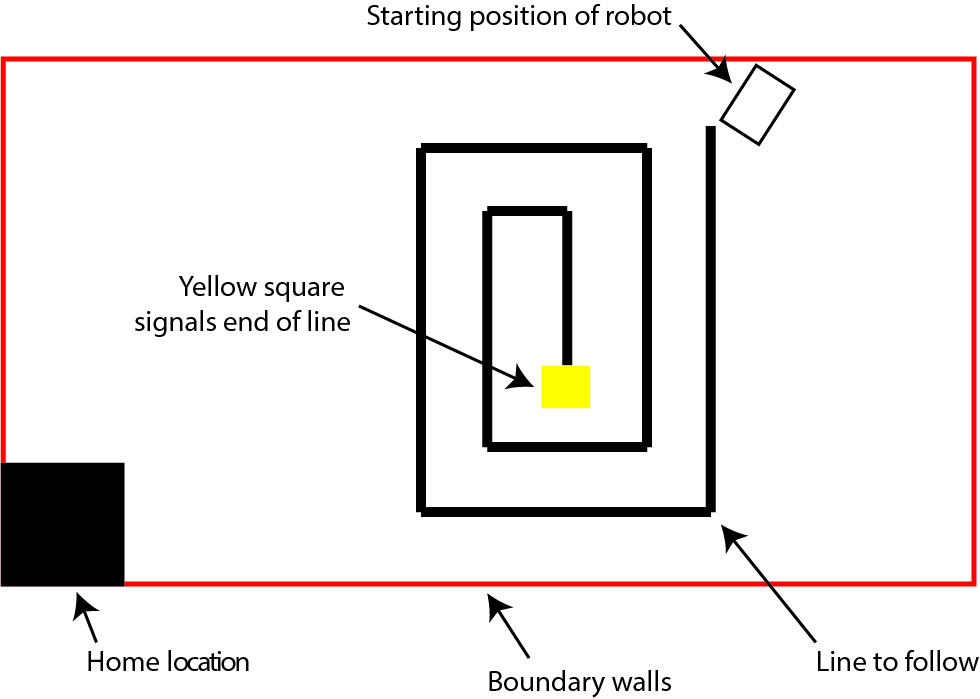
\includegraphics[width=1\columnwidth]{field.jpg}\\
  \caption{The test field is rectangular, with a solid black line for the robot to follow. The end of the black line is marked by a solid yellow square. The home location is designated by the solid black square in the lower left corner.}
  \label{F.field}
\end{figure}

The hardware required for this challenge includes two light sensors, a color sensor and a sound sensor. The light sensors are used to measure reflected light which helps the robot differentiate between the white field and the black line, the color sensor is used to sense the yellow card which marks the end of the line, and the sound sensor is used to tell when the crowd is cheering the robot in the right direction. 

The sensors are arranged such that one of the light sensors is on each side of the line at all times, and the color sensor is mounted in the center of the robots path so that it will pass over the yellow square. The sound sensor on the other hand is mounted high above the NXT so that it is located closer to the crowd and also to mitigate the effect of motor noises.

Figure~\ref{F.hardware} shows the location and orientation of each of the sensors. Because the robot always turns right along the line, the right and left light sensors are offset slightly as shown to avoid getting stuck on a turn. When the sensors are directly beside each other, the potential exists for the left sensor to run over the corner at the same time the right sensor is tripped. This results in the robot thinking that a line is running across the front of it which can cause it to get stuck.

\begin{figure}[ht]
 \centering
  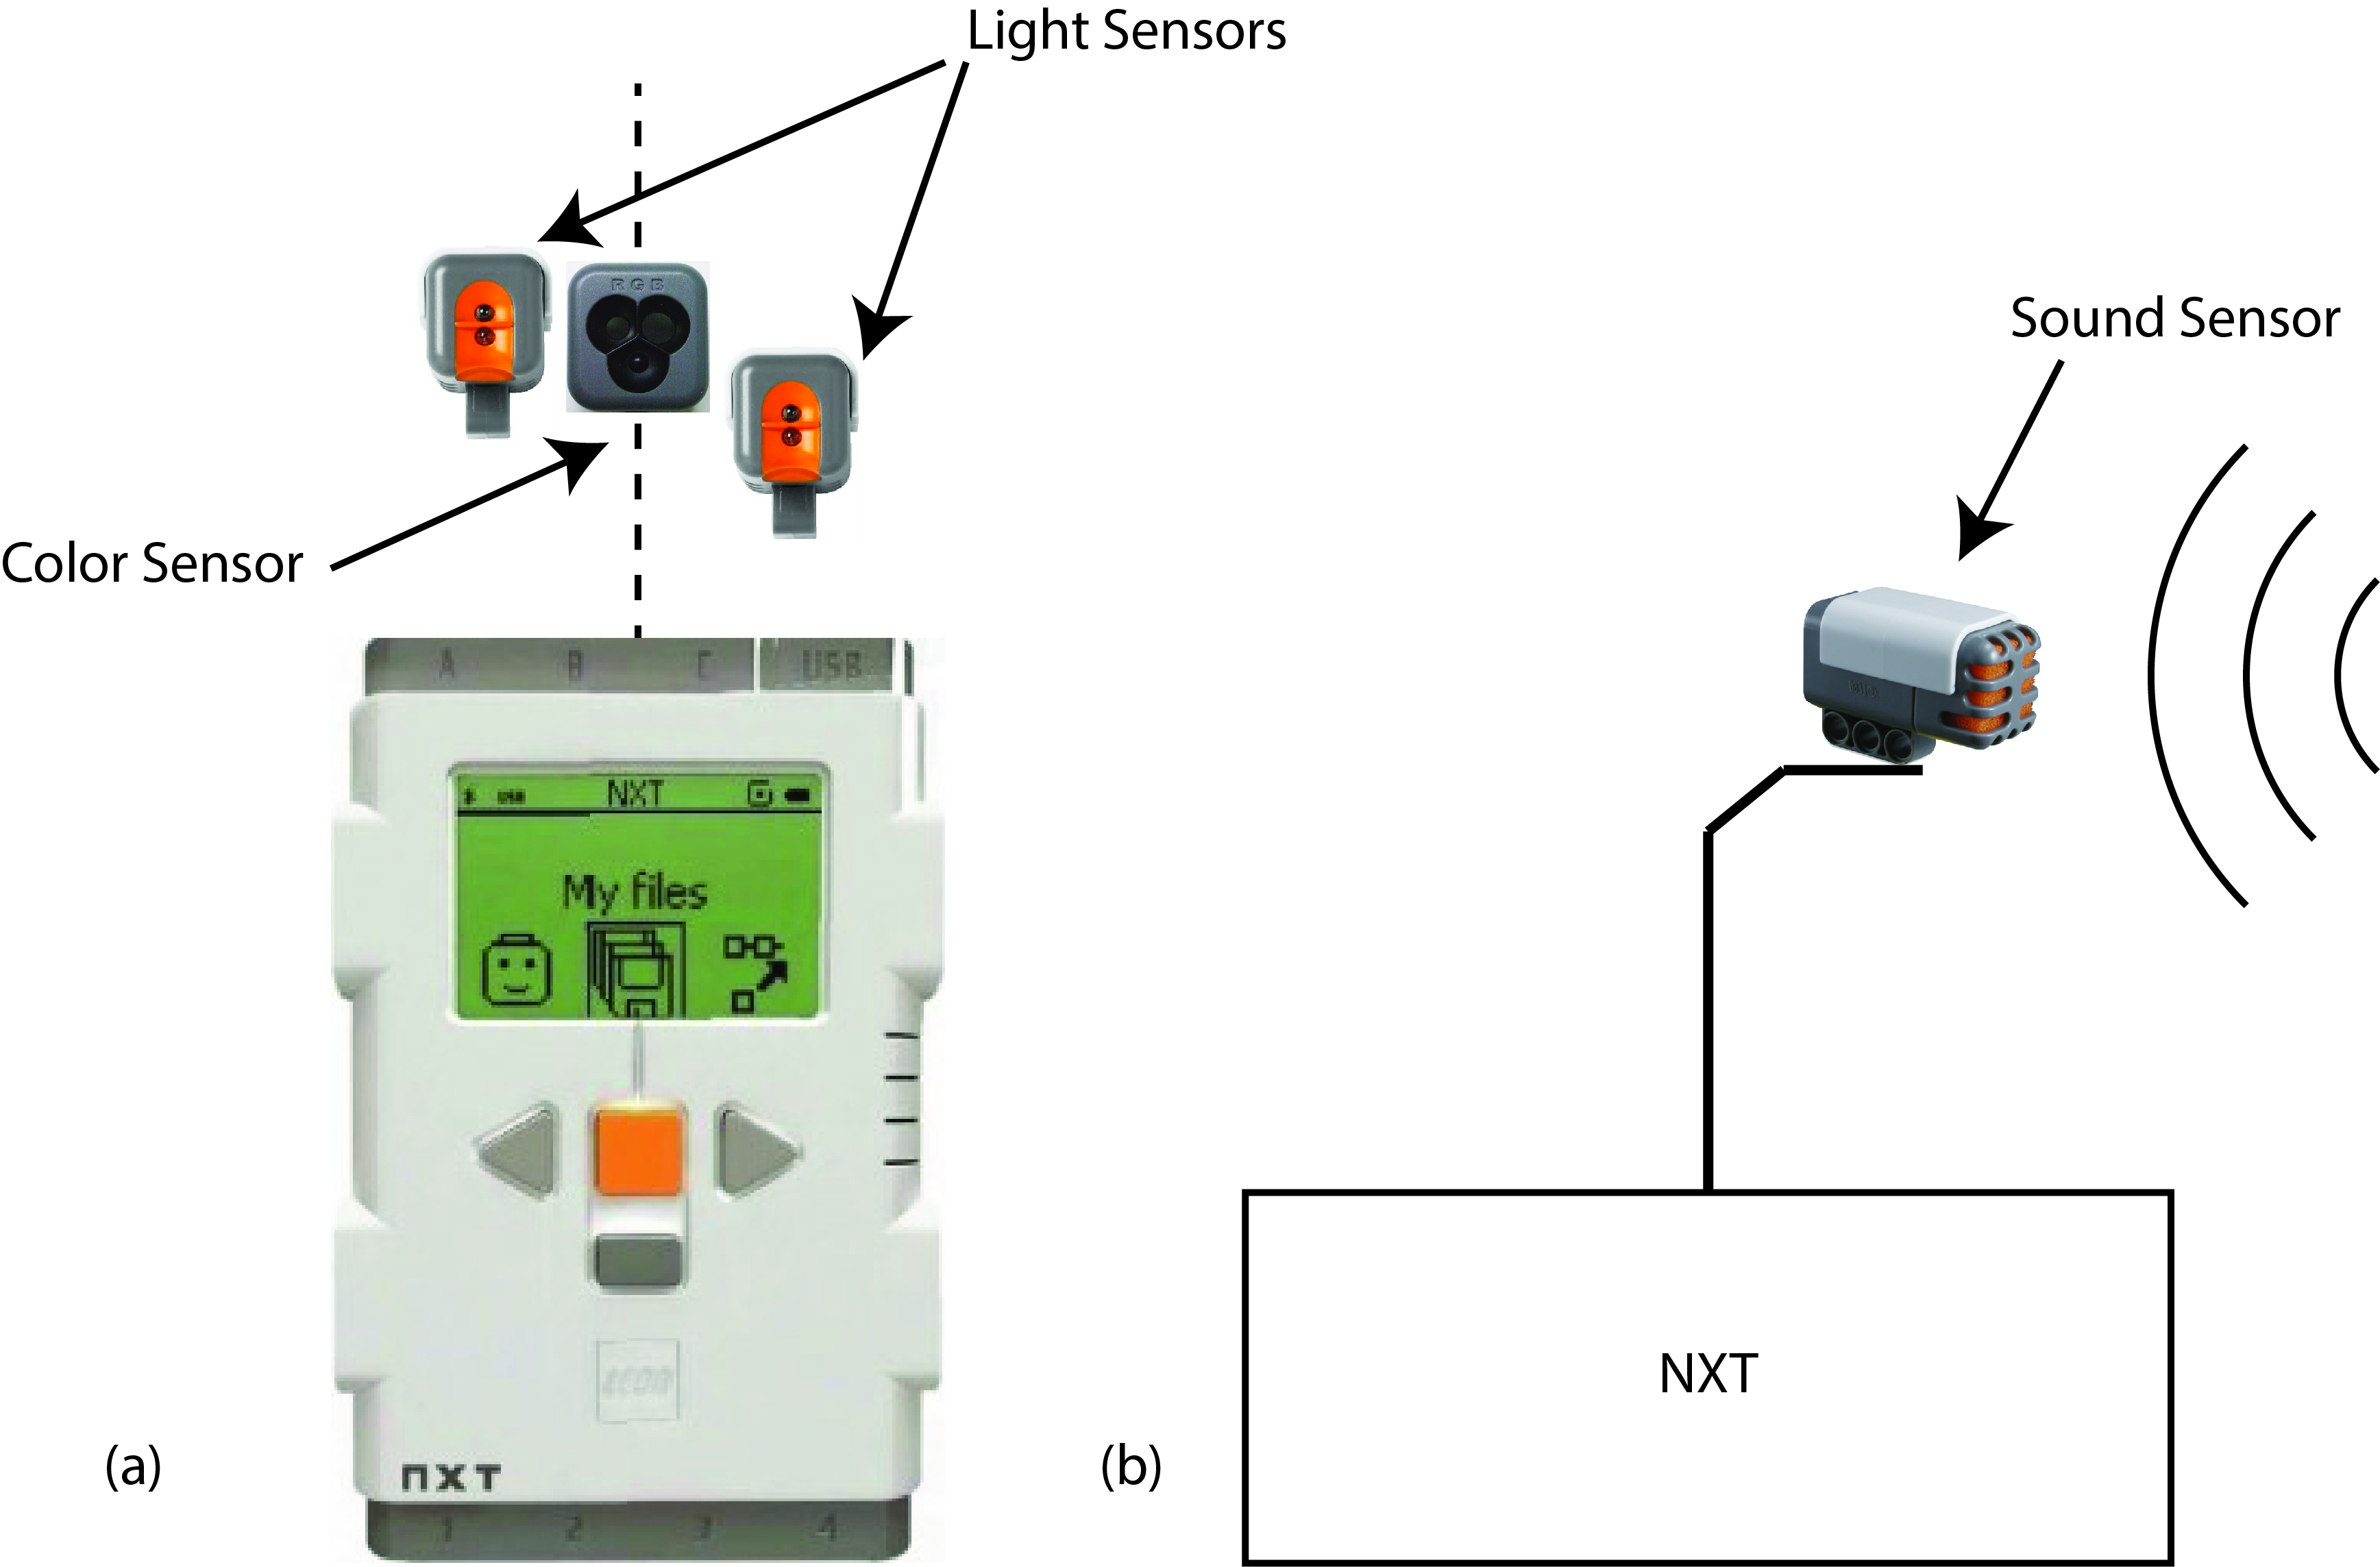
\includegraphics[width=1\columnwidth]{hardware.jpg}\\
  \caption{The overall hardware design is shown from the top view (a) and the side view (b). Note that the light sensors are slightly offset front to back to favor left hand turns.}
  \label{F.hardware}
\end{figure}

The software design for this challenge is a sequence broken into three specific portions. First, because the robot does not start directly on the line it must find it. Next, the robot should follow the line until it reaches the yellow card. Finally, the robot should seek out its home location based on cheering directions from the crowd.

The first part of the program is the method of finding the line. We know which direction the robot will approach the line from, so we tell the robot to move forward until the left sensor sees the line at which point it should turn left until the right sensor has passed over the line once. In all cases, this will result in the robot being centered on the line, and oriented in the right direction. 

During the line following portion of the program, the robot monitors the left and right light sensors and adjust the motor powers based on the readings. The motor powers depend only on the corresponding left or right sensor and are proportionally controlled according to the relationship 

\begin{equation}\label{E.motor_speed}
    P_{motor} = \frac{P_{max}-P_{min}}{I_{max}-I_{min}}I_{sensor} + offset
\end{equation}

where $P_{motor}$ is the calculated motor power, $P_{max}$ and $P_{min}$ are the maximum and minimum power settings for the motors (user configureable), $I_{max}$ and $I_{min}$ are the maximum and minimum sensed values (experimentally determined), and $I_{sensor}$ is the value that the sensor is currently reading. The offset for this equation can easily be calculated in software using all of the user configurable parameters, and the experimentally determined sensor limits by

\begin{equation}\label{E.motor_speed}
    offset = P_{max} - \frac{P_{max}-P_{min}}{I_{max}-I_{min}}I_{max}.
\end{equation}

The result of these power settings is that the motor speeds increase when further away from the line and decrease and even reverse (if $P_{min}$ is less than zero) when the sensor gets closer to the line. The behavior that this produces in the robot is that the motor speed incrementally decreases as it approaches a line slowly, but when it reaches a corner the power is immediately decreases to its minimum in order to complete the turn. 

All throughout the line following portion of the challenge, the robot is monitoring the color sensor to determine if it has reached the end of the line. This is accomplished by running the line following code in a while loop which terminates when the color sensor reads the appropriate value for yellow.

The final part of the challenge is for the robot to find home based on cheering from the crowd. The software used to implement this simply monitors the sound sensor and has two actions. When the noise threshold is below a user configurable value, the robot spins in place but when the noise level is above the threshold, the robot drives in a straight line. This effectively allows the crowd to steer the robot by being quite in order to orient in the correct direction and then cheering to move it straight ahead. Of course, the robot does not drive completely straight, so this process may need to be attempted multiple times before reaching the home location.

\section{Problems Encountered}\label{S.problems}

There were several significant problems with this lab. Our previous front end mounting for the sensor array took up too much space, was too complicated, and put unnecessary strain on the Lego parts. We iterated through several possible new arrangements before finding one that met these requirements.

When initially devising a line traversal strategy, we discovered that the robot would have severe difficulty navigating a corner. The sonsors would arrive at an even blck line simultaneously, causing our algorithm to stop the motors and halt the robot entirely, or would overshoot the line and escape. 

In arriving at a new arrangement for our sensor array, we discovered that the light sensors, the sensors responsible for guiding the robot along the line, became drastically less sensitive. We attempted several software-based solutions for this, mostly varying our constants for contrast sensitivity, but no software configuration worked.

We had extreme difficulty utilizing the multiplexer as required by the lab. It seems that it is not well documented and there were few coding examples which did not cover the entirety of the proper usage. It also had difficulties using certain types of sensors, which we discovered through trial and error. This was also undocumented.

The specific requirements of the lab stated that the robot was to identify the home square with the color sensor, however, due to the nature of the shape and color line to be followed, it would be extremely difficult to determine the difference between the home square and the line. This might cause the robot to either potentially stop when it reached a portion of the line, mistaking it for the home square, or if some delay were to be added, mistaking the home square for the line and continuing perpetually.


\section{Solutions}\label{S.solutions}

When initially testing the algorithm, we discovered that arranging the right sensor slightly behind the relative position of the left one caused the robot to turn along the line path. This allowed us to not only use the algorithm we had already designed, but to exploit the specific design of the line with a bias toward turning to the right. If the line had spiraled counter-clockwise, in order to use the same algorithm the left sensor would have to have been behind the right one causing a bias to turn toward the left.

We discovered that the light sensors were more sensitive to the contrast between the background and the line in a certain orientation. There appears to be a slight notch in the red light beam emitted by the sensors which appears to indicate a blind spot in the sensors' vision. The arrangement of the sensors we originally used oriented this blind spot on both sensors toward the line. Rearranging the sensors so that the sensitive side opposite the blind spot were facing the line solved this problem and restored the functionality of following the line we observed prior to changing our sensor array arrangement.

Our professor was kind enough to waive the requirement that the robot visually identify the home square, instead allowing piloting entirely through the sound sensor. This allowed us to focus on learning how to anticipate the movements of the robot in its home-finding circling and grasp the timing required to get the robot to move forward at appropriate times.

\section{Unsolved Problems}\label{S.unsolved}

We managed to utilize a few sensors through the multiplexer using what example code we could find, but noticed a significant delay in the responsiveness of the sensors attached to it. This eliminated the light sensors as candidates as the responsiveness became so low that the robot would overshoot the line by a significant margin or ignore it almost entirely. Ultimately only the sound sensor was connected to the multiplexer as this was the only sensor that could afford to be delayed while being compatible and maintaining a level of performance.

\end{document}
